\documentclass[lettersize,journal]{IEEEtran}
\usepackage{amsmath,amsfonts}
\usepackage{algorithmic}
\usepackage{algorithm}
\usepackage{array}
\usepackage[caption=false,font=normalsize,labelfont=sf,textfont=sf]{subfig}
\usepackage{textcomp}
\usepackage{stfloats}
\usepackage{url}
\usepackage{verbatim}
\usepackage{graphicx}
\usepackage{cite}
\hyphenation{op-tical net-works semi-conduc-tor IEEE-Xplore}

\begin{document}

\title{An EDA of Recruitment Data}

\author{Saakar K.C,\hspace{1mm}Student,\hspace{1mm}Kathmandu University}
\maketitle
    
\begin{abstract}
Exploratory Data Analysis (EDA) has evolved into a pivotal process, essential for conducting initial investigations into data and unraveling relationships among explanatory variables. EDA serves as a fundamental tool for gaining a deeper understanding of data, pinpointing errors, identifying outliers or irregularities, and validating assumptions. In today's fiercely competitive market, the recruitment of top-notch talent from diverse backgrounds is paramount to an organization's success. To fully leverage the potential of a given dataset, this report encapsulates and scrutinizes it to unearth valuable insights and discern patterns that can guide strategic, data-driven decision-making in the realm of talent acquisition. Furthermore, this report underscores the significance of data-driven decision-making in the field of talent acquisition, offering valuable insights to HR professionals and line managers.
\end{abstract}

\begin{IEEEkeywords}
EDA,Knowledge Discovery in Database
\end{IEEEkeywords}

\section{Introduction}
\IEEEPARstart{E}{xploratory} Data Analysis (EDA) is one of the techniques used for extracting vital features and trends used by machine learning and deep learning models in Data Science. Thus, EDA has become an important milestone for anyone working in data science. This article covers the concept, meaning, tools, and techniques of EDA to give complete awareness to a beginner wanting to launch a career in data science. The article also enlists those fields that regularly apply EDA efficiently in promoting their business activities.  


\section{Methodology}
Based upon Knowledge Discovery in Database(KDD) which refers to the process of discovering useful information, patterns and  knowledge from large volumes of data.KDD encompasses various steps, including data preprocessing, data cleaning ,data transformation,data mining and interpretation of results.For this the tools that are used are Jupyter Notebook and orange.

\section{Data Exploration}
Exploration, one of the first steps in data preparation, is a way to get to know data before working with it. Through survey and investigation, large data sets are readied for deeper, more structured analysis.\\
\hspace{5mm} This data set includes 3000 instances and 18 attributes with 9 feature and 9 meta attributes.No missing data is found in the data set but attribute Phone Number is found to have no data with some of the rows having hashtags instead of the number.\\
The 9 features are Application ID,
Application Date, Gender, State, Zip Code, Education Level, Years of Experience, Desired Salary and Status while meta attributes include First Name, Last Name, Date of Birth, Phone Number, Email, Address, City, Country and Job Title.\\ For handling noisy data I found dataset  with mist distinct values and the nominal attributes like State, Country, City, Zip Code and
Address.\\

In general, the ordering of attributes in \textbf{Figure 1} would be like address \textless zip code \textless city \textless state \textless country but here in our data set the attribute State contains 59 states and territories of the United States with its abbreviation[5]. The country attributes include all countries present while it does n’t match up with corresponding cities. So only considering State attributes. \\
Data reduction techniques can be applied to obtain a reduced representation of the data set that is much smaller in volume yet maintains the integrity of the original data . Also, the Age attribute is calculated from the applicant's Date of Birth and Application Date. So, the final obtained data set includes an Application ID, application date, Gender, State, Educational level, years of experience, Desired Salary, Job Title, Status and Age.


\begin{figure}[t]
\centering
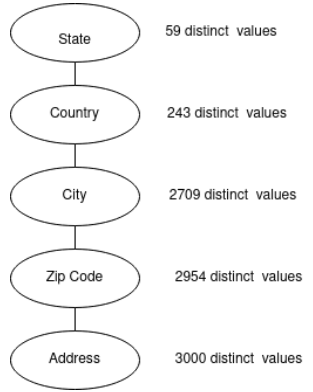
\includegraphics[width=2.5in]{Screenshot 2023-09-08 142035.png}
\caption{Nominal Attributes}
\label{fig_1}
\end{figure}

\section{Univariate Non-Graphical EDA}
Univariate Non-Graphical Exploratory Data Analysis (EDA) involves analyzing a single variable or attribute in a dataset without using visualizations or graphs. Instead, it focuses on summary statistics and other quantitative methods to gain insights into the characteristics of that variable.
\subsection{Categorical Data}
Categorical data, also known as qualitative data, is a type of data that represents categories or labels, rather than numerical values. It is used to group data into distinct categories or classes, and it is often used to describe characteristics or attributes that do not have a natural numerical order.


\subsubsection{Gender}
In \textbf{fig-2}, the count and percentage of all three genders are nearly equal which helps in gender diversity in a office environment.


\begin{figure}[h]
\centering
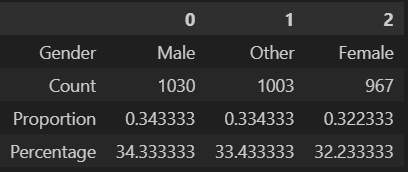
\includegraphics[width=2.5in]{Screenshot 2023-09-08 151203.png}
\caption{Tabulation of gender attribute}
\label{fig_2}
\end{figure}

\subsubsection{Status}
In \textbf{Figure 3}, the applicants are equally distributed across different statuses. These observations can provide valuable insights to HR professionals as they work on improving the hiring process and implementing strategies to efficiently allocate new employees throughout the organization's management structure.

\begin{figure}[h]
\centering
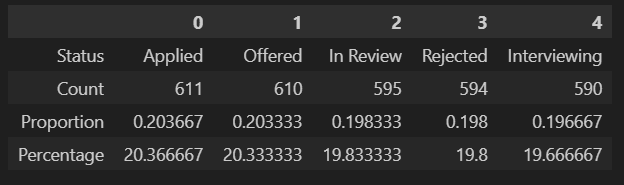
\includegraphics[width=2.5in]{Screenshot 2023-09-08 152511.png}
\caption{Tabulation of status attribute}
\label{fig_3}
\end{figure}


\subsubsection{Education Level}
Tabulation of fig 4 possesses a diverse range of
educational levels which will provide valuable insights for
recruitment strategies


\begin{figure}[h]
\centering
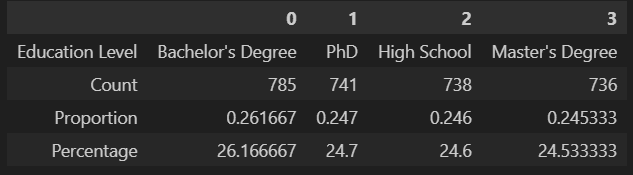
\includegraphics[width=2.5in]{Screenshot 2023-09-08 153027.png}
\caption{Tabulation of Education Level attribute}
\label{fig_4}
\end{figure}

\subsection{Numeric Data}
This includes calculation of mean, variance, quartiles,
minimum value and maximum values.
\subsubsection{Years of Experience}
 For population of 3000 instances
 \begin{list}{}{}  
\item[ µ = 9.96 years]
\item[ $\sigma$ = 6.03]
\item [Q1 = 5]
\item[ Q3 = 15]
\item[ min. = 0 year]
\item[  max. = 20 years]
\end{list}

\subsubsection{Desired Salary}
\begin{list}{}{}
\item[ µ =0163.05 amount]
\item[$\sigma$ =20163.67 amount]
\item[Q1 = 47307.80]
\item[Q3 = 82585.59]
\item[min. = 300047.22]
\item[max. = 99992.66]
\end{list}
    

\subsubsection{Age}
\begin{list}{}{}
\item[N = 3000]
\item[µ = 39.39]
\item[$\sigma$ = 12.47]
\item[Q1 = 29]
\item[Q3 = 50]
\item[min. = 17]
\item[max. = 60]
\end{list}


\section{Bivariate Non-graphical EDA}
Bivariate data arises from more than one variable. Bivariate non-graphical EDA techniques generally show the relationship between two or more variables of the data through cross-tabulation or statistics
\subsection{Categorical Data}
Categorical data, also known as qualitative data or nominal data, is a type of data that represents categories or labels rather than numerical values. It is used to classify or group data into distinct categories, with each category representing a different attribute or characteristic

\subsubsection{Gender and Education level}

From figure 4, among females the most common
educational level is “Bachelor’s Degree”, for males and other
the distribution is nearly equal.
\begin{figure}[h]
\centering
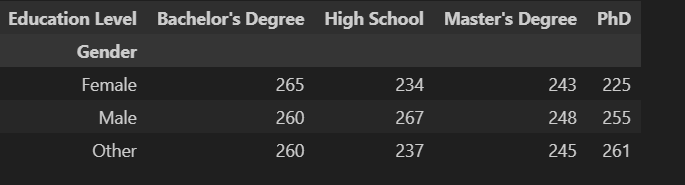
\includegraphics[width=3.5in]{Screenshot 2023-09-08 155959.png}
\caption{Cross Tabulation between Gender and Educational Level}
\label{fig_4}
\end{figure}

\subsubsection{Gender and Status}

From figure 5 must male apply for jobs and their
distribution is nearly equal and other gender is also relatively
balanced

\begin{figure}[h]
\centering
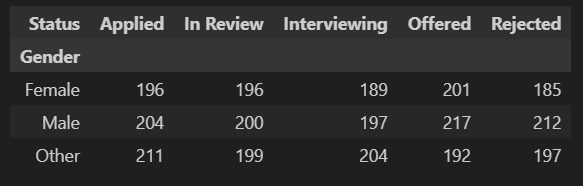
\includegraphics[width=3.5in]{Screenshot 2023-09-08 160134.png}
\caption{Cross Tabulation between Gender and Status}
\label{fig_5}
\end{figure}

\subsubsection{Status and Education Level}
Following table ca be obtained from the dataset 
\begin{figure}[h]
\centering
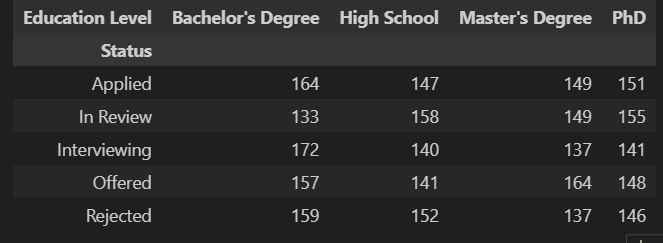
\includegraphics[width=3.5in]{Screenshot 2023-09-08 160141.png}
\caption{Cross Tabulation between Status and Education Level}
\label{fig_6}
\end{figure}
\pagebreak
\subsection{Numeric Data}
The Pearson correlation between attributes are:
\begin{enumerate}
    \item{ +0.027 between Desired Salary and Years of Experience.}
    \item{-0.02 between Age and Year of Experience}
    \item{-0.002 between Age and Desired Salary}
\end{enumerate}
    


\section{Univariate Graphical EDA}
This includes bar-plot,box plot, and histogram
\subsection{Years of Experience}

\begin{figure}[h]
\centering
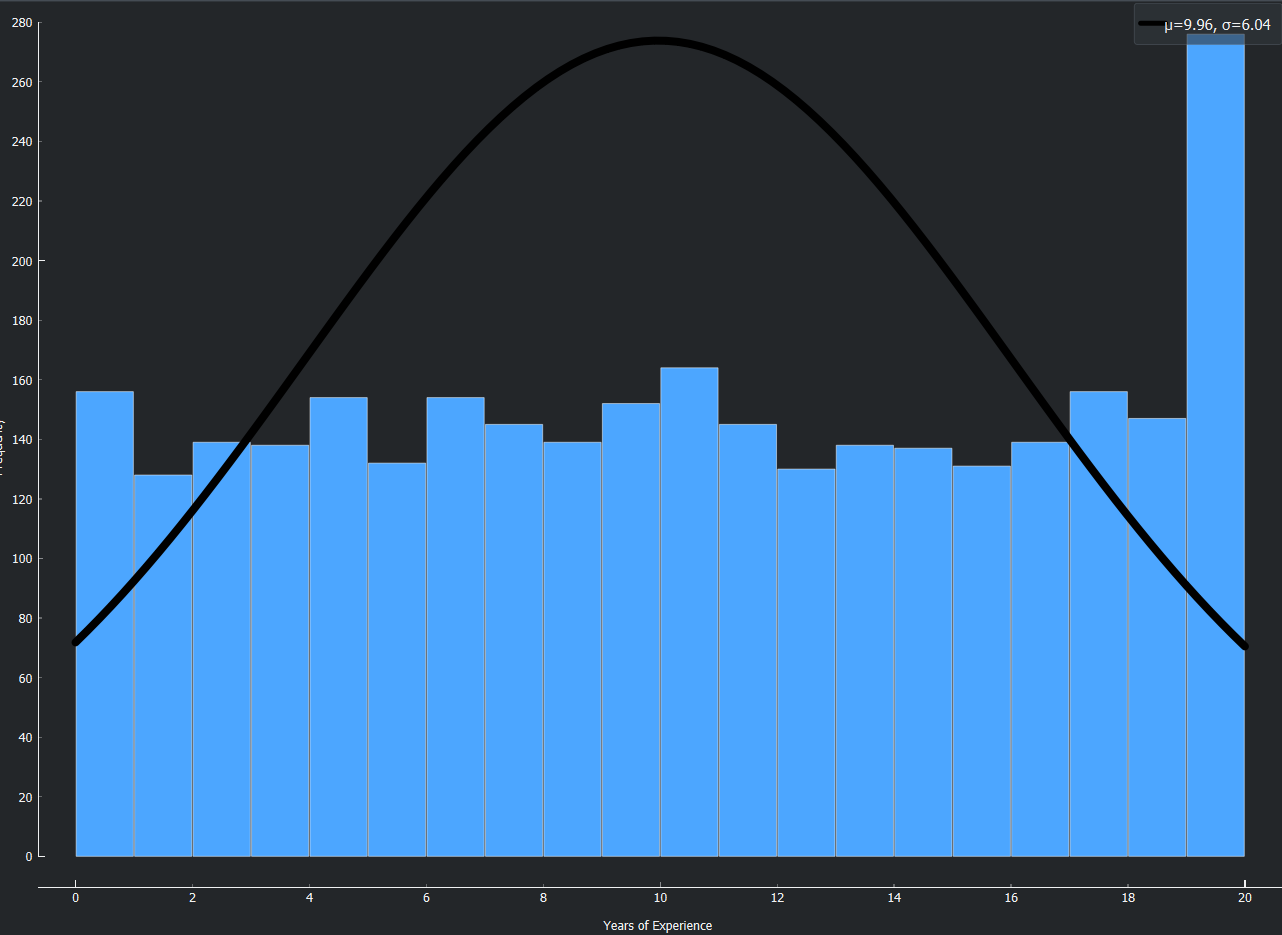
\includegraphics[width=3.5in]{histrogram.png}
\caption{Years of experience in histogram}
\label{fig_5}
\end{figure}

\begin{figure}[h]
\centering
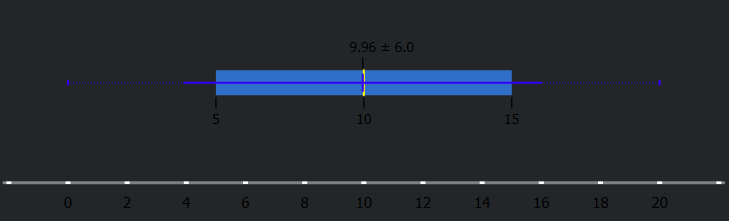
\includegraphics[width=3.5in]{boxpot.png}
\caption{Years of experience in boxplot}
\label{fig_5}
\end{figure}

\subsection{Desired Salary}
This show the desired salary of all candidates in  and in box-plot diagram
\vspace{28mm}

\begin{figure}[h]
\centering
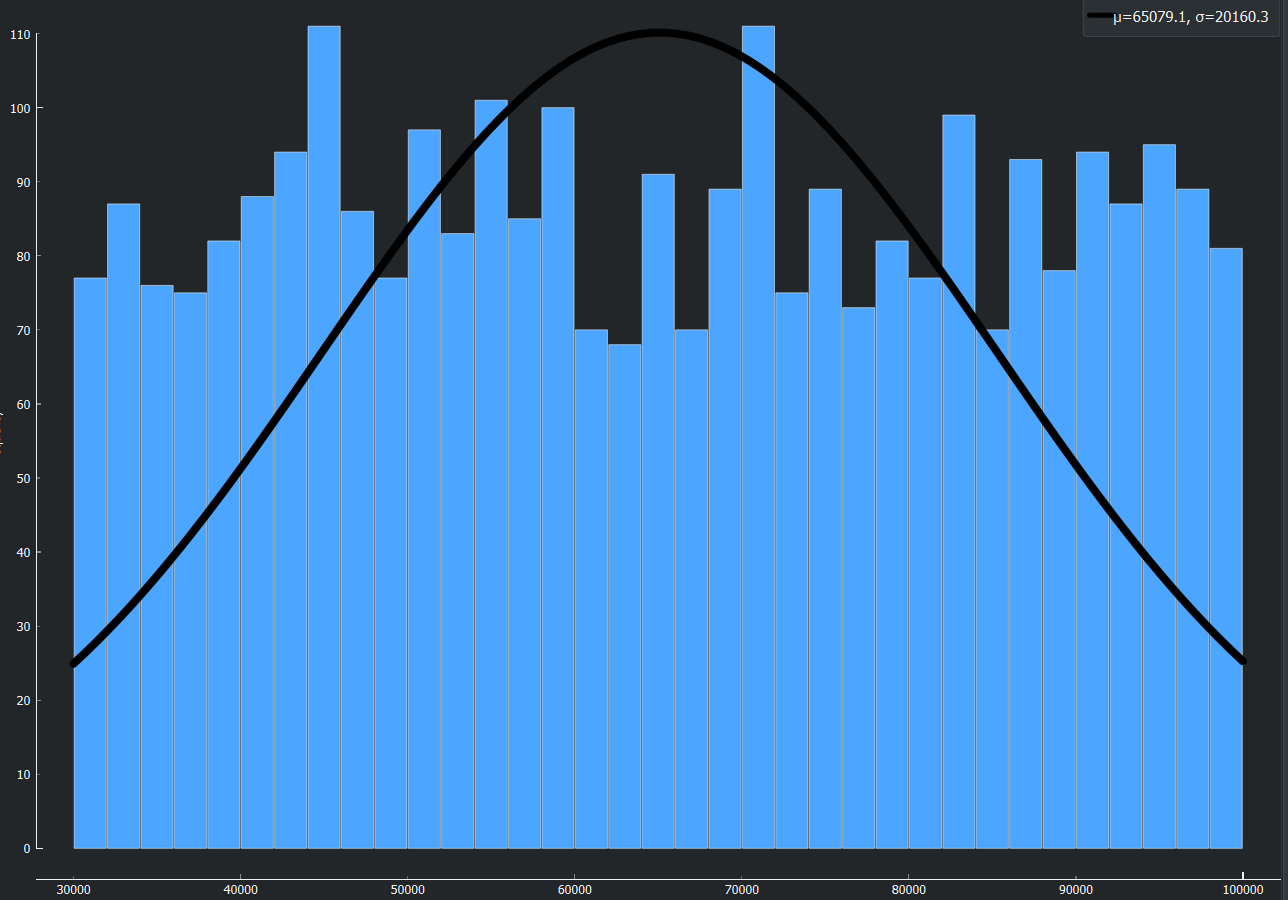
\includegraphics[width=3.5in]{dshistrogram.png}
\caption{Desired Salary in histogram}
\label{fig_5}
\end{figure}

\begin{figure}[h]
\centering
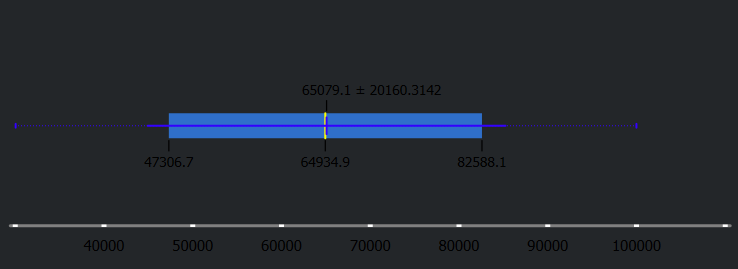
\includegraphics[width=3.5in]{dsboxplot.png}
\caption{Desired Salary in box-plot}
\label{fig_5}
\end{figure}

\subsection{Age}
This shows the age of all the candidates in histrogram and in Box-plot diagram.
\vspace{15mm}

\begin{figure}[h]
\centering
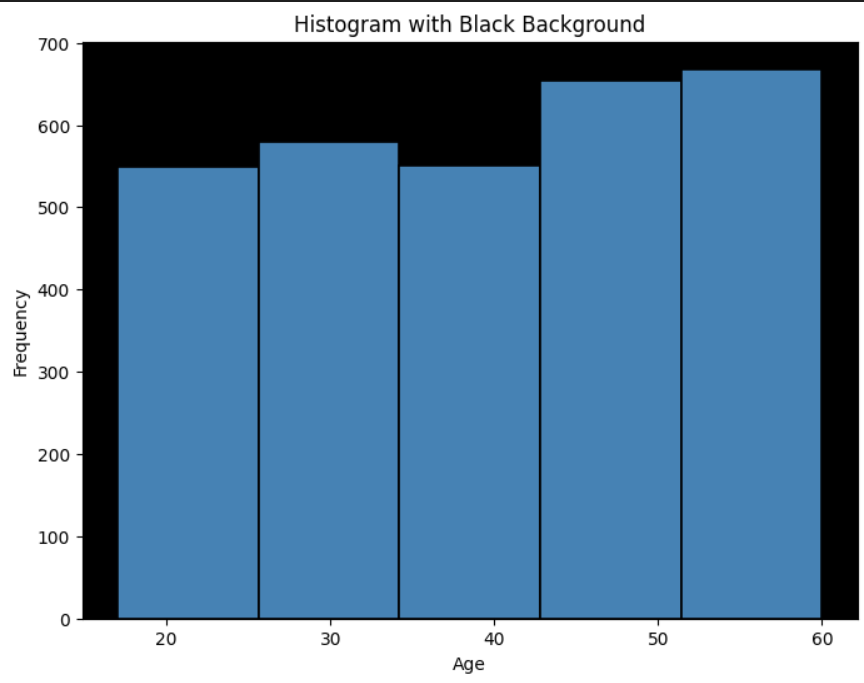
\includegraphics[width=3.5in]{ageh.png}
\caption{Age in histogram}
\label{fig_5}
\end{figure}

\begin{figure}[h]
\centering
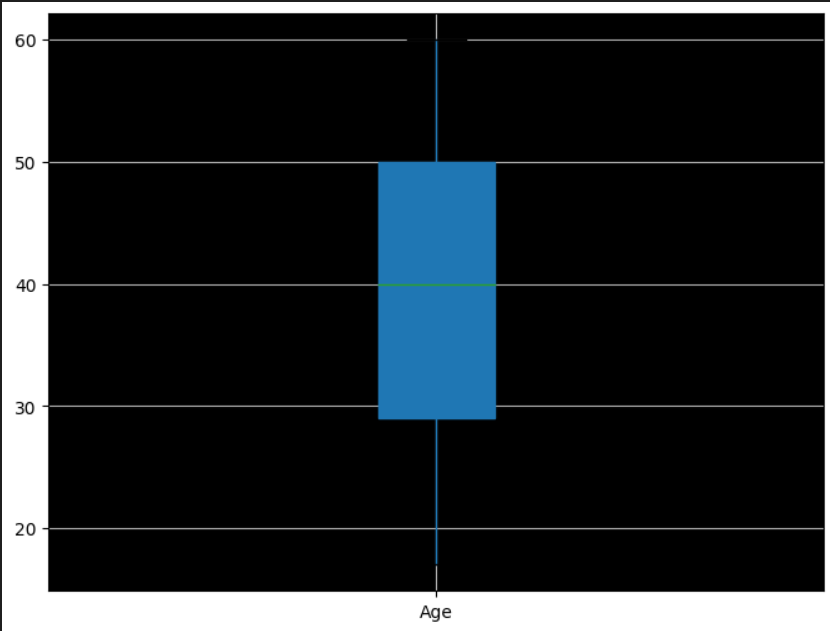
\includegraphics[width=3.5in]{agebox.png}
\caption{Age in box-plot}
\label{fig_5}
\end{figure}
\section{Bivariate Graphical EDA}

Bivariate data uses graphics to display relationships
between two sets of data. The most used graphics is a grouped
bar plot or bar chart.

\subsection{Categorical Data}
Bivariate Graphical Exploratory Data Analysis (EDA) with categorical data involves using visual techniques to understand the relationships and patterns between two categorical variables.
These methods help reveal associations, dependencies, and insights within categorical data sets

\vspace{5mm}

\subsubsection{Education and Status }
 From fig 14 most applicants who applied for a job
hold a bachelor's degree while most of the applicants only got
High School diplomas and the distribution seems evenly
distributed.
\vspace{5mm}
\begin{figure}[h]
\centering
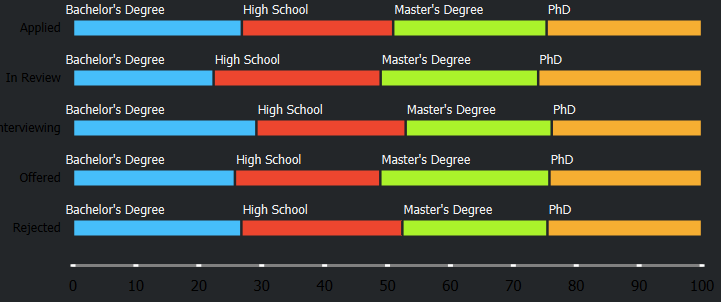
\includegraphics[width=3.5in]{Screenshot 2023-09-08 175042.png}
\caption{Education level and Status BOX-Plot}
\label{fig_14}
\end{figure}
 
\vspace{5mm}
\subsubsection{Gender and education Level}

\begin{figure}[h]
\centering
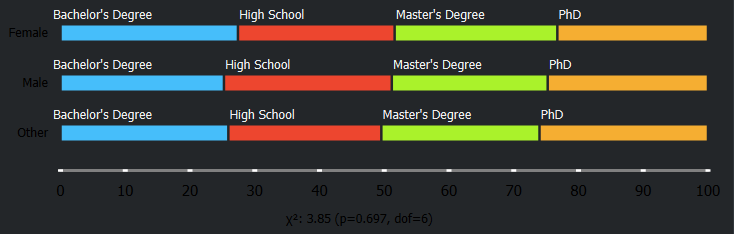
\includegraphics[width=3.5in]{Screenshot 2023-09-08 175337.png}
\caption{Gender and Education Level}
\label{fig_14}
\end{figure}

fig 15 Educational level and Gender bar plot
From fig 7.1.2, among females the most common
educational level is “Bachelor’s Degree”, for males and other
the distribution is nearly equal.

\subsection{Numerical Data}
\subsubsection{Year of Experience and Desired Salary }


\begin{figure}[h]
\centering
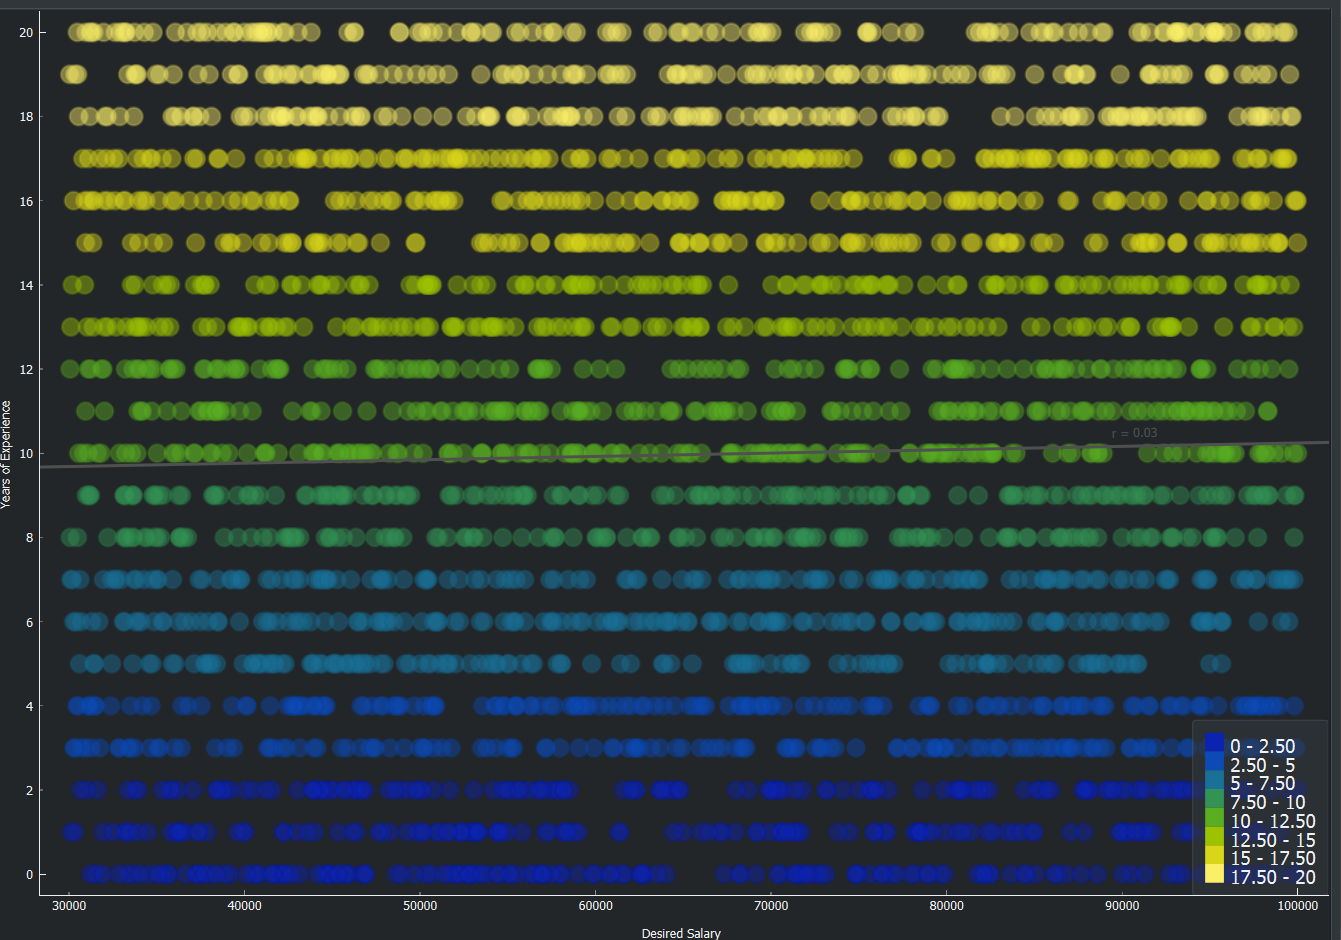
\includegraphics[width=3.5in]{scatterplot1.png}
\caption{Year of Experience and Desired Salary in Scatter Plot}
\label{fig_14}
\end{figure}

From Fig 16 the correlation value is r = 0.03 which
shows the weak relationship between these attributes. In
general, the correlation should be positive as an increase in
Years of Experience tends to increase Desired Salary. The
value r=0.02 suggests there is a weak positive linear
relationship
 
\section{Conclusion}
Exploratory Data Analysis (EDA) plays a crucial role in the assessment of recruitment data, shedding light on the balanced distribution of applicants across various educational levels and highlighting the significance of fostering a diverse and inclusive workforce. This analysis underscores that the hiring process is unbiased with regard to gender, emphasizing the organization's commitment to equality in talent acquisition.

\section*{Acknowledgement}
The author wishes to express gratitude to Assistant Professor Rajani Chulyadyo at Kathmandu University for her invaluable guidance and expertise during the data mining course.

\end{document}


